\chapter{Tecnologie e strumenti}
\label{chap:tecnologie_strumenti}
Di seguito verranno dettagliate le tecnologie, gli strumenti, i framework ed i linguaggi impiegati nello sviluppo del progetto.
\section{Aulos}
\label{chap:aulos}
\begin{figure}[h]
\begin{center}
  
\includegraphics[width=5cm]{images/aulos_logo.png}
  \caption{Logo di AULOS}
\end{center}
\end{figure}
AULOS è il \textit{framework} utilizzato all'interno dell'impresa Loccioni per standardizzare lo sviluppo e rendere riconoscibile e uniforme lo stile grafico di applicativi per la visualizzazione dati. La parte frontend utilizza la tecnologia Angular, mentre la parte backend può essere scritta utilizzando linguaggi come C\# e LabView.\\
Un componente fondamentale sul quale si è basato il lavoro svolto per il progetto è la \textit{dashboard}, nata dall'esigenza di monitorare in tempo reale i dati provenienti dalle macchine Loccioni. Offre un ambiente di \textit{authoring} che permette ai clienti di creare ad hoc in maniera semplice e veloce il proprio pannello personalizzabile \cite{AULOS}.
La dashboard è composta da:
\begin{itemize}
    \item l'elenco di tutti i possibili widget selezionabili dall'utente;
    \item la griglia centrale in cui l'utente può selezionare, spostare, ridimensionare o eliminare un widget;
    \item il pannello di configurazione, che si attiva selezionando un widget e permette all'utente di andare a modificare le impostazioni legate a esso.
\end{itemize}
\begin{figure}[h]
\begin{center}
  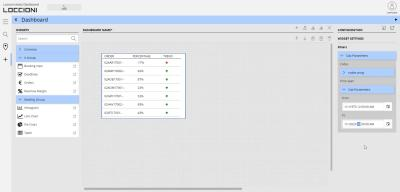
\includegraphics[width=14cm]{images/dashboard_aulos.JPG}
  \caption{Dashboard del framework AULOS}
\end{center}
\end{figure}
\pagebreak
Il \textit{widget}, attore principale all'interno della dashboard,
è una mini applicazione che permette all'utente di visualizzare dati e svolgere semplici azioni. Nel progetto discusso ne sono stati sviluppati diversi relativi ai dati generati dalle macchine e ai flussi gestionali interni all'impresa.
\begin{figure}[h]
\begin{center}
  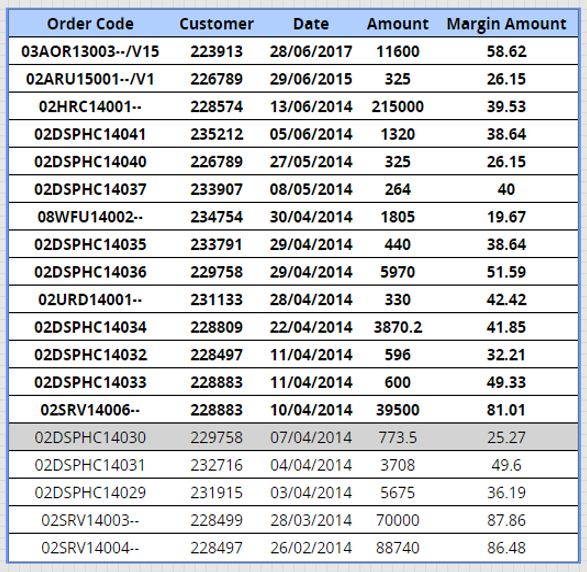
\includegraphics[width=7cm]{images/orders_widget.jpg}
  \caption{Widget realizzato per la visualizzazione degli ordini}
\end{center}
\end{figure}
\paragraph{Storybook}
AULOS offre una pagina di \textit{storybook} al fine di agevolare gli sviluppatori nell'utilizzo dei suoi componenti. Ciascuna storia contenuta al suo interno si occupa di descrivere tutti gli stati di \textit{rendering} interessanti di un componente UI e di fornirne una spiegazione implementativa \cite{STORYBOOK}.
\pagebreak
\begin{figure}[h]
\begin{center}
  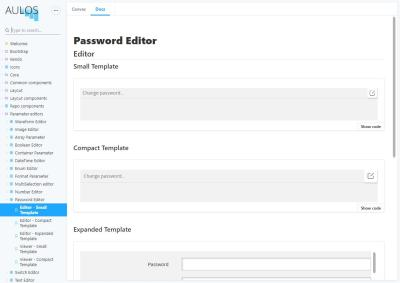
\includegraphics[width=14cm]{images/aulos_storybook.JPG}
  \caption{Vista sullo storybook del framework AULOS}
\end{center}
\end{figure}

\section{Angular 10}
\begin{figure}[ht!]
\begin{center}
  
\includegraphics[width=7cm]{images/angular_logo.png}
  \caption{Logo Angular}
\end{center}
\end{figure}
\FloatBarrier
\textit{L'applicativo frontend} del progetto discusso nella tesi è stato sviluppato con Angular.
Angular è una piattaforma e un framework per costruire applicazioni \textit{client single-page} usando i linguaggi HTML e TypeScript \cite{ANGULAR}. 
\paragraph{HTML} HTML (Hypertext Markup Language) è il \textit{linguaggio di markup} standard per i documenti visualizzabili in un browser web \cite{HTML}.
\paragraph{TypeScript} TypeScript è un linguaggio di programmazione \textit{open source} sviluppato da Microsoft. Estende la sintassi di JavaScript, essendo un suo superset, in modo che qualunque programma scritto in JavaScript sia anche in grado di funzionare con TypeScript senza nessuna modifica. È stato progettato per lo sviluppo di grandi applicazioni ed è destinato a essere compilato in JavaScript per poter essere interpretato da qualunque web browser o app. \cite{TYPESCRIPT}
L'architettura di un'applicazione Angular si basa su alcuni concetti fondamentali. Gli elementi costitutivi di base sono gli \textit{NgModules}, che forniscono un contesto di compilazione per i \textit{Component}. Questi ultimi sono elementi fondamentali per la costruzione delle UI in Angular. Ciascun Component definisce una classe che contiene dati e logica dell'applicazione ed è associato ad un modello HTML che definisce come verrà visualizzato nell'ambiente di destinazione. Il decoratore \textit{@Component()} identifica la classe immediatamente sotto di essa come un componente e fornisce il modello e i relativi metadati specifici del componente.
I decoratori sono funzioni che modificano le classi JavaScript. Angular definisce un numero di decoratori che associano specifici tipi di metadati alle classi, in modo che il sistema sappia cosa significano quelle classi e come dovrebbero funzionare.\cite{ANGULAR}
\begin{lstlisting}[caption={Esempio di un Component in Angular}, style=javaScriptCode]
import { Component, OnInit } from '@angular/core';
@Component({
  selector: 'app-root',
  templateUrl: './app.component.html'
})
export class AppComponent implements OnInit {

  constructor() { }

  ngOnInit() { }

}
\end{lstlisting}
Per i dati o la logica che non sono associati a una vista specifica e che si desidera condividere tra i componenti si crea una classe di servizio. Una definizione di classe di servizio è immediatamente preceduta dal decoratore \textit{@Injectable()}. Il decoratore fornisce i metadati che consentono ad altri provider di essere inseriti come dipendenze nella classe.
La \textit{dependency injection (DI)} consente di mantenere le classi dei componenti snelle ed efficienti. Esse non recuperano dati dal server, convalidano l'input dell'utente o accedono direttamente alla console; delegano tali compiti ai servizi. \cite{ANGULAR}
\begin{lstlisting}[caption={Esempio di un Service in Angular}, style=javaScriptCode]
import { Injectable } from '@angular/core';
import { HttpClient } from '@angular/common/http';
import { Observable } from 'rxjs';
import { Data } from '...';

@Injectable({
  providedIn: 'root',
})
export class AppService {

  constructor( private http: HttpClient, private url: string ) { }
  
  public getData(): Observable<Data[]> {
    return this.http.get<Data[]>(this.url);
  }

}
\end{lstlisting}
Per la gestione interna dei pacchetti in Angular è stato utilizzato \textit{npm} (node package manager), un gestore di pacchetti per il linguaggio di programmazione JavaScript. È il gestore di pacchetti predefinito per l'ambiente di runtime JavaScript \textit{Node.js}. Consiste in un client da linea di comando, chiamato anch'esso npm, e un database online di pacchetti pubblici e privati, chiamato \textit{npm registry}.
Il registry è accessibile via client e i pacchetti disponibili sono consultabili sul sito web di npm. \cite{NPM}

\section{RxJs}
\begin{figure}[h!]
\begin{center}
  
\includegraphics[width=7cm]{images/RxJs.png}
  \caption{Logo RxJs}
\end{center}
\end{figure}
RxJS (\textit{Reactive Extensions for JavaScript}) è una libreria per la programmazione reattiva \footnote{La programmazione reattiva è un paradigma di programmazione asincrona che riguarda i flussi di dati e la propagazione del cambiamento.} che utilizza \textit{Observable}, che semplifica la composizione di codice asincrono o basato su \textit{callback}. RxJS fornisce un'implementazione di \textit{Observable} e funzioni di utilità al fine di lavorarci. \cite{RxJS} 

Queste ultime possono essere utilizzate per:
\begin{itemize}
    \item convertire codice esistente per operazioni asincrone in \textit{Observable};
    \item iterare sui valori di uno stream;
    \item mappare valori di diversi tipi;
    \item filtrare stream;
    \item effettuare la composizione di più stream.
\end{itemize}

\section{KendoUI}
\begin{figure}[ht!]
\begin{center}
  
\includegraphics[width=6cm]{images/kendo_logo.png}
  \caption{Logo Kendo UI}
\end{center}
\end{figure}
Kendo UI è un framework integrale di interfaccia utente HTML5 per costruire applicazioni e siti web interattivi e ad alte prestazioni. \cite{KENDO}
Il framework è stato usato all'interno dell'applicativo frontend con l'obiettivo di conferire un aspetto grafico più accattivante ai widget. Kendo UI per Angular offre un vasto numero di componenti.

\begin{figure}[h!]
\begin{center}
  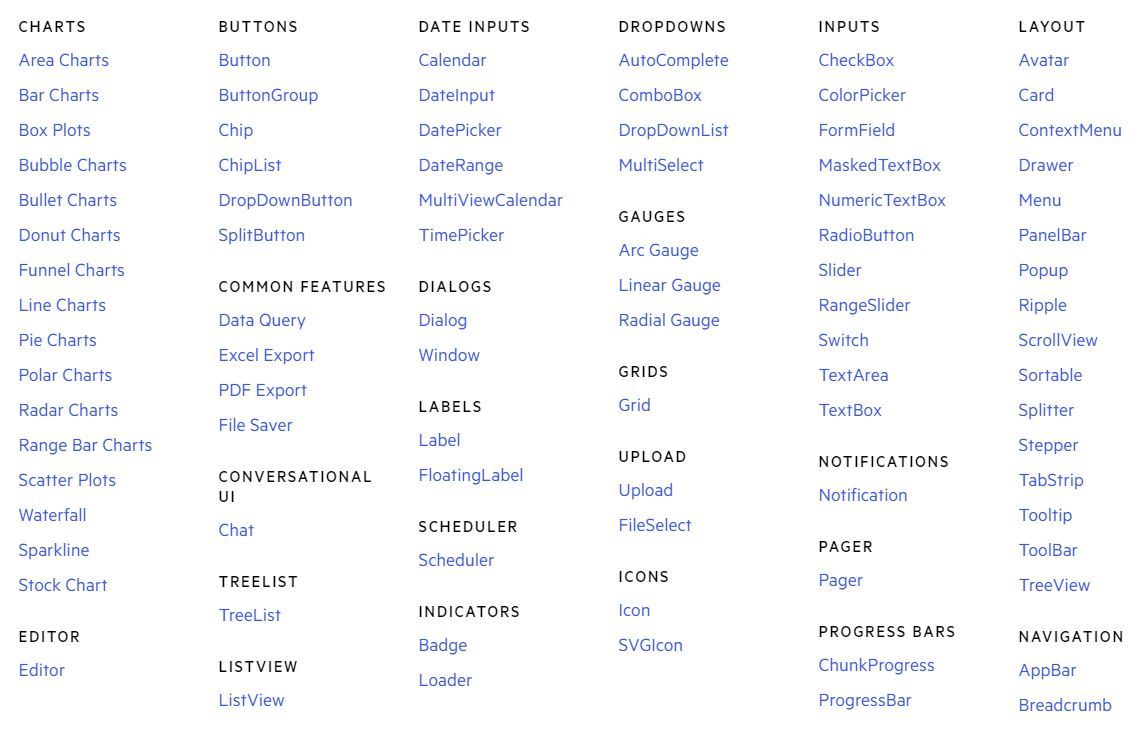
\includegraphics[width=15cm]{images/kendo_components.JPG}
  \caption{Componenti di Kendo UI per Angular}
\end{center}
\end{figure}
\pagebreak
Ogni componente include un set completo di funzionalità già pronte all'uso \cite{KENDO}. Nel caso della \textit{Kendo Grid}, componente frequentemente utilizzato nel progetto per rappresentare dei dati all'interno di una tabella, vi è ad esempio la possibilità di filtrare, ordinare, modificare e raggruppare i dati agevolmente.
\begin{figure}[ht!]
\begin{center}
  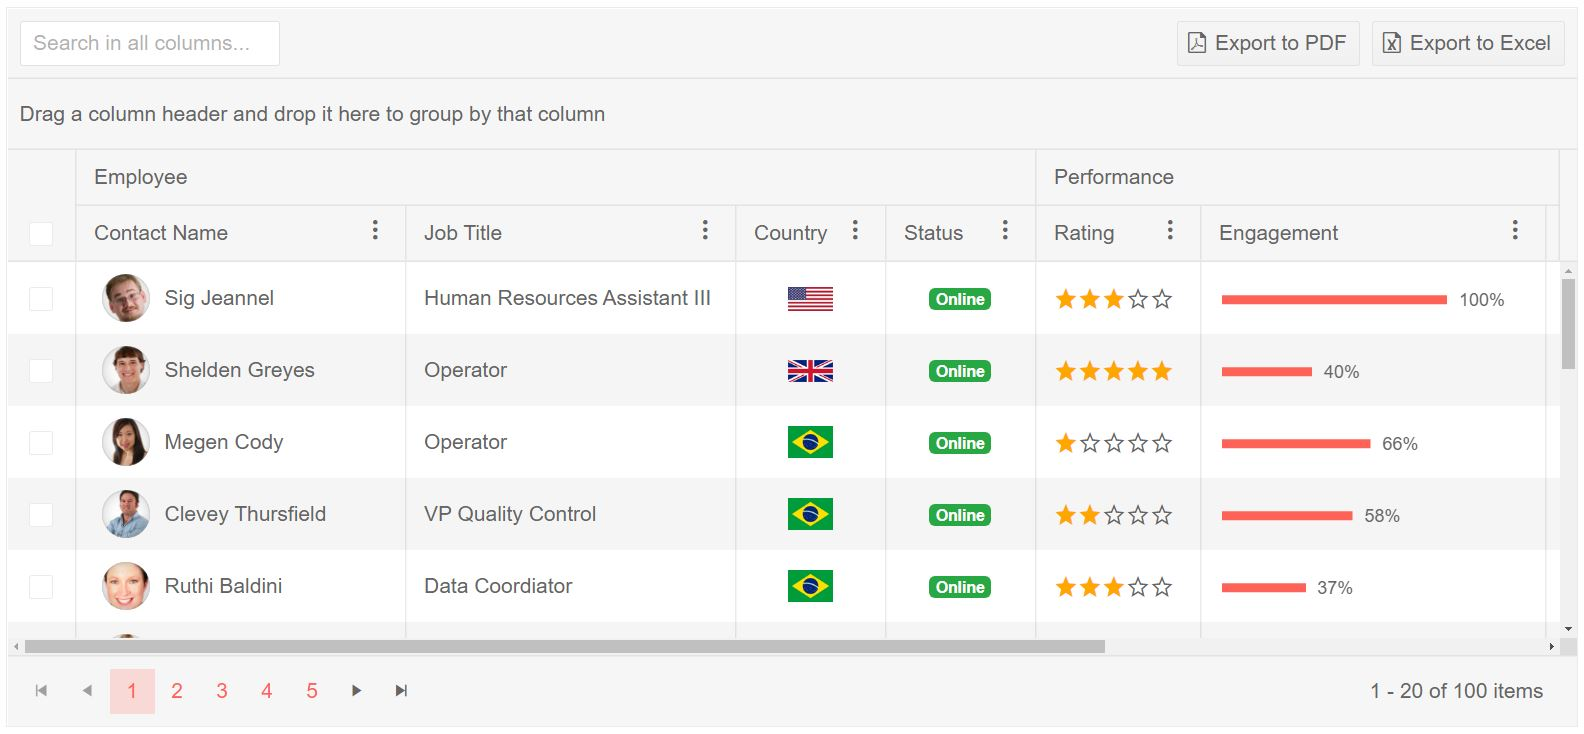
\includegraphics[width=14cm]{images/kendo_grid.JPG}
  \caption{Esempio di Kendo Grid per Angular}
\end{center}
\end{figure}

\pagebreak
\section{.NET}
\begin{figure}[h!]
\begin{center}
	
\includegraphics[width=7cm]{images/dotnet.png}
	\caption{Logo di .NET}\label{fig:dotnet}
\end{center}
\end{figure}
.NET è una piattaforma di sviluppo ideata da Microsoft per costruire differenti tipi di applicazioni, utilizzando il C\#, F\# o Visual Basic.\cite{DOTNET} 
\begin{itemize}
\item \textbf{C\#} è un linguaggio di programmazione object-oriented semplice, moderno e fortemente tipizzato;
\item \textbf{F\#} è un linguaggio di programmazione funzionale \textit{cross-platform} e \textit{open-source}. Include anche tratti di programmazione imperativa e object-oriented;
\item \textbf{Visual Basic} è un linguaggio di programmazione intuitivo con una sintassi semplice volto a scrivere app object-oriented e fortemente tipizzate.
\end{itemize}
Viene divisa in due versioni principali:
\begin{itemize}
\item \textbf{.NET Core} è la versione cross-platform, e viene utilizzata per lo sviluppo di siti, servizi e console apps. È questa la versione che è stata utilizzata nello sviluppo dell'applicativo backend;
\item \textbf{.NET Framework} è la versione solo per Windows, e viene utilizzata per lo sviluppo di ogni tipo di app che può essere eseguita di Windows.
\end{itemize}
\pagebreak
\subsection{ASP.NET}
\begin{figure}[h]
\begin{center}
	
\includegraphics[width=7cm]{images/aspnet.png}
	\caption{ASP.NET}\label{fig:aspnet}
\end{center}
\end{figure}
ASP.NET è un framework di sviluppo open-source per web applications lato server. È stato sviluppato da Microsoft per permettere ai programmatori di costruire pagine web dinamiche, applicazioni e servizi.\cite{ASPNET}\\
Analogamente a .NET, presenta due versioni:
\begin{itemize}
\item \textbf{ASP.NET Core} è la versione cross-platform che utilizza il runtime di .NET Core;
\item \textbf{ASP.NET Core 4.x} è la versione solo per Windows che utilizza il runtime di .NET Framework.
\end{itemize}

\subsection{Entity Framework}
\begin{figure}[h]
\begin{center}
	
\includegraphics[width=7cm]{images/entityframework.png}
	\caption{Entity Framework}\label{fig:entityframework}
\end{center}
\end{figure}
Entity Framework è un ORM framework (Object-relational mapping) per .NET supportato da Microsoft. Permette agli sviluppatori di lavorare con i dati usando oggetti specifici del dominio senza concentrarsi sulle tabelle e colonne dei database in cui sono memorizzati i dati.
\subsection{Entity Framework Core}
Entity Framework Core è una versione leggera, estensibile, open source e cross-platform di Entity Framework. È stato utilizzato per lavorare con i dati del progetto memorizzati in server SQL e MySQL \cite{EF}.

\pagebreak
\section{Linq}
\label{sec:linq}
\begin{figure}[ht!]
\begin{center}
  
\includegraphics[width=4.5cm]{images/linq.png}
  \caption{Logo LINQ}
\end{center}
\end{figure}
LINQ (Language-Integrated Query) è il nome di un set di tecnologie basate sull'integrazione delle funzionalità di query direttamente nel linguaggio C\#. In genere, le query sui dati vengono espresse come stringhe semplici senza il controllo dei tipi in fase di compilazione o il supporto IntelliSense. È anche necessario imparare un linguaggio di query diverso per ogni tipo di origine dati: database SQL, documenti XML, svariati servizi Web e così via. Con LINQ, una query è un costrutto del linguaggio di prima classe, come le classi, i metodi e gli eventi. È possibile scrivere query su insiemi di oggetti fortemente tipizzati usando le parole chiave del linguaggio e gli operatori comuni. La famiglia di tecnologie LINQ offre coerenza per l'esecuzione di query per oggetti (LINQ to Objects), database relazionali (LINQ to SQL) e XML (LINQ to XML). Per uno sviluppatore che scrive query, la parte integrata nel linguaggio più visibile di LINQ è l'espressione di query. Le espressioni di query vengono scritte con una sintassi di query dichiarativa. Tramite la sintassi di query è possibile eseguire operazioni di filtro, ordinamento e raggruppamento sulle origini dati usando una quantità minima di codice \cite{Linq}.

\section{ElasticSearch}
\begin{figure}[ht!]
\begin{center}
  
\includegraphics[width=6cm]{images/esearch.png}
  \caption{Logo ElasticSearch}
\end{center}
\end{figure}
Elasticsearch è un motore di ricerca e analisi full-text open source altamente scalabile. Consente di archiviare, cercare e analizzare grandi volumi di dati rapidamente e quasi in tempo reale. Viene generalmente utilizzato come motore sottostante per applicazioni che hanno caratteristiche e requisiti di ricerca complessi.
Elasticsearch dispone di diversi casi d'uso \cite{ELASTICSEARCH}:
\begin{itemize}
    \item consente di avere una visione più ampia delle informazioni a disposizione senza risultare dispersivo, anche con agglomerati di dati estremamente consistenti grazie alle ``aggregazioni'';
    \item combina diversi tipi di ricerche: strutturate, non strutturate, geografiche, ricerca di applicazioni, analisi della sicurezza, metriche e registrazione;
    \item si adatta a qualsiasi situazione che va dal semplice computer con un singolo nodo fino ad arrivare a un cluster con centinaia di server, rendendo la creazione di un prototipo più agevole;
    \item utilizza API RESTful standard e JSON. L'apporto costante della comunità ha portato alla creazione e al mantenimento di client in molti linguaggi come Java, Python, .NET, SQL, Perl, PHP;
    \item è possibile utilizzare le funzionalità di ricerca e analisi in tempo reale di Elasticsearch per lavorare sui big data utilizzando il connettore Elasticsearch-Hadoop (ES-Hadoop).
\end{itemize}
Data l'elevata efficienza di questo software diverse compagnie informatiche l'hanno scelto per i loro prodotti. Gli ambiti interessati sono quelli di ricerca per quanto concerne \textit{Tinder}, dove Elasticsearch permette di rendere il sistema più reattivo e veloce, mentre nel caso di \textit{Netflix} l'utilizzo principale è focalizzato al giusto indirizzamento di notifiche push, email e messaggistica \cite{ELASTICSEARCH}.
Nel progetto discusso, Elasticsearch è stato utilizzato nell'implementazione del layer di accesso dei dati relativi alle macchine che testano le componenti degli elettrodomestici \textit{Whirlpool}. In sinergia con questo strumento è stata impiegata la dashboard di visualizzazione dati \textit{Kibana}.

\section{Nest}
\begin{figure}[ht!]
\begin{center}
  
\includegraphics[width=6cm]{images/elastic.png}
  \caption{Logo Elastic}
\end{center}
\end{figure}
NEST è un client Elasticsearch .NET di alto livello che è ancora molto fedele all'API Elasticsearch originale. Tutte le richieste e le risposte sono esposte attraverso i tipi, rendendolo ideale per essere subito operativi.
Tutti i metodi disponibili all'interno di NEST sono esposti sia come versioni sincrone che asincrone, con queste ultime che utilizzano suffisso idiomatico \textit{Async} sul nome del metodo \cite{Nest}.
Di seguito la medesima richiesta effettuata in Postman utilizzando un payload in formato json~\ref{fig:json} e in Nest~\ref{fig:nest}.
\pagebreak
\begin{figure}[ht!]
\begin{center}
  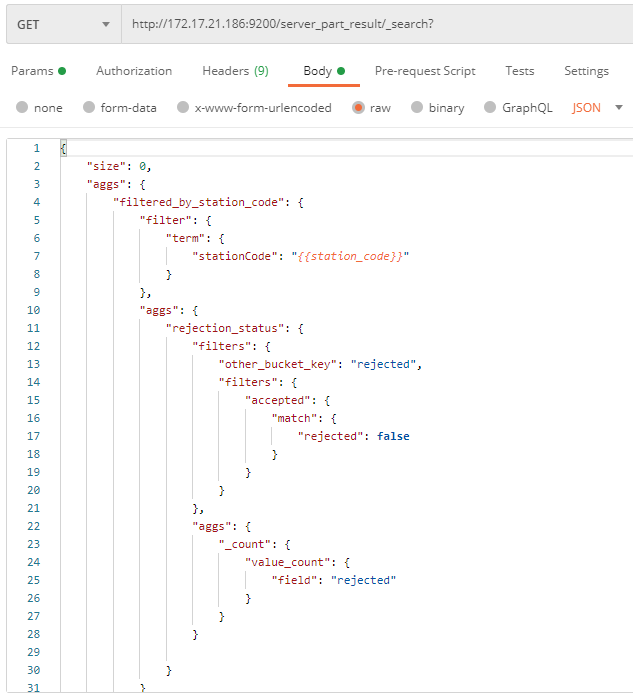
\includegraphics[width=11cm]{images/json.png}
  \caption{Query in json}
  \label{fig:json}
\end{center}
\end{figure}
\begin{figure}[ht!]
\begin{center}
  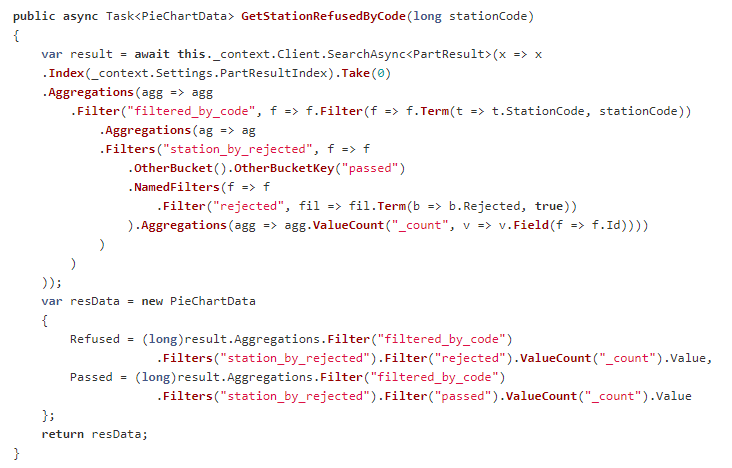
\includegraphics[width=12cm]{images/NestQuery.PNG}
  \caption{Query in Nest}
  \label{fig:nest}
\end{center}
\end{figure}

\section{Newtonsoft JSON}
\begin{figure}[ht!]
\begin{center}
  
\includegraphics[width=8cm]{images/newtonsoft.png}
  \caption{Newtonsoft JSON.NET}
  \label{fig:newtonsoft}
\end{center}
\end{figure}
JSON.NET è un framework open source di gestione JSON per framework .NET che mette a disposizione funzionalità di serializzazione e deserializzazione di oggetti .NET, manipolazione di JSON utilizzando sintassi LINQ (Sec.~\ref{sec:linq}), query su JSON utilizzando sintassi pseudo-XPath \cite{XPATH}, elevata performance relativamente alle librerie di serializzazione incluse in .NET e conversione XML-JSON.\footcite{NEWTONSOFT}

\section{Git}
\begin{figure}[ht!]
\begin{center}
  
\includegraphics[width=5cm]{images/git_logo.jpg}
  \caption{Logo Git}
\end{center}
\end{figure}
Git è un software di controllo versione distribuito utilizzabile da interfaccia a riga di comando. \cite{GIT}
Un software di controllo versione è un'applicazione che permette di tenere traccia di tutti gli aggiornamenti apportati ad uno specifico progetto software, o \textit{repository}.
Oltre a mostrare una visione più generale e strutturata sul progetto, Git consente agli sviluppatori di implementare codice in team nella maniera più efficiente possibile riducendo i conflitti che possono nascere da uno sviluppo parallelo. Questo viene reso possibile grazie ad un sistema a rami, dall'inglese \textit{branches}, che permettono allo sviluppatore di lavorare in autonomia in uno spazio completamente isolato dal resto del progetto. Per riunificare poi il nuovo codice implementato con il branch principale, lo sviluppatore potrà effettuare un'operazione di \textit{merge}.
\begin{figure}[ht!]
\begin{center}
  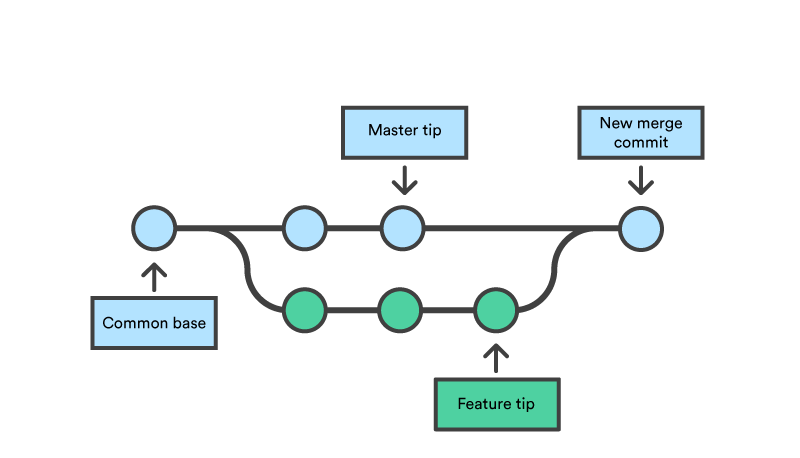
\includegraphics[width=12cm]{images/merge-di-due-branch.png}
  \caption{Esempio di merge di due branch in Git}
\end{center}
\end{figure}

\pagebreak
\section{Gitlab}
\begin{figure}[ht!]
\begin{center}
  
\includegraphics[width=7cm]{images/gitlab_logo.png}
  \caption{Logo GitLab}
\end{center}
\end{figure}
GitLab è una piattaforma web open source che permette la gestione di repository Git e di funzioni trouble ticket \cite{GITLAB}.
La piattaforma si basa sull'offrire uno spazio virtuale remoto, pubblico o privato, dove archiviare il proprio repository, permettendo agli sviluppatori di lavorare in team.
Inoltre GitLab consente di avere un controllo più immediato mettendo a disposizione dello sviluppatore una vista sui branch creati e una history delle modifiche apportate al repository.
Ulteriore funzionalità è quella dei trouble ticket, ovvero le \textit{issue} all'interno di GitLab. Questo sistema consente di creare dei ticket per richiedere agli sviluppatori di aggiungere nuove funzionalità o di risolvere uno specifico bug. Una volta soddisfatta la richiesta il ticket potrà essere chiuso e disattivato dallo sviluppatore.
\begin{figure}[ht!]
\begin{center}
  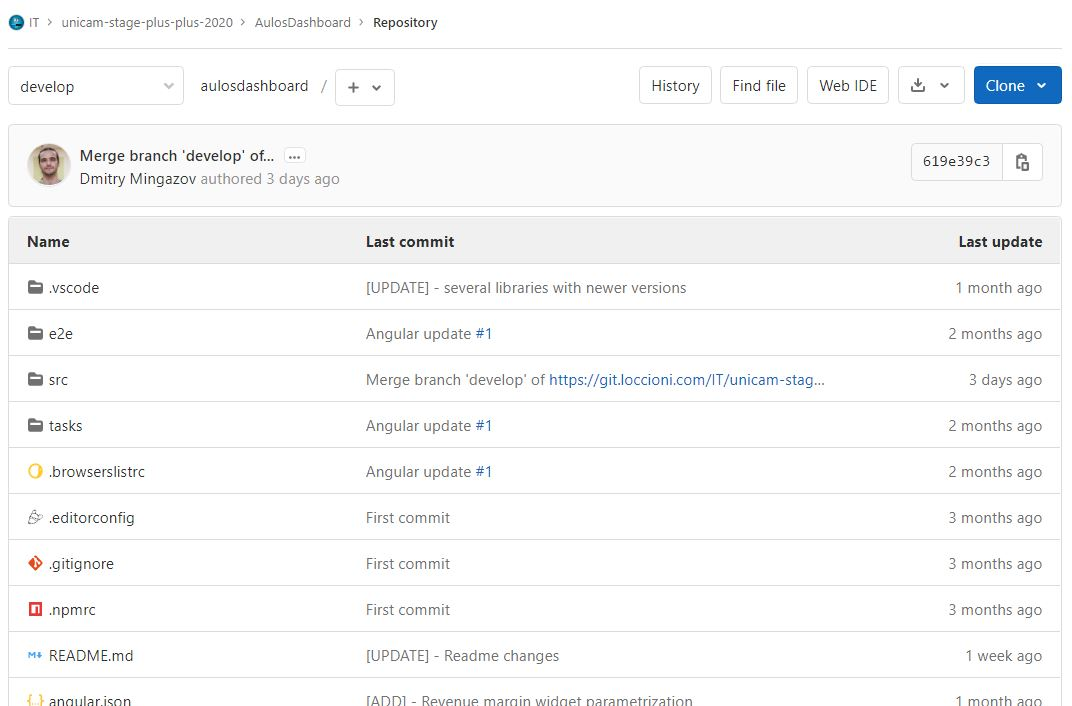
\includegraphics[width=13cm]{images/Repository_GitLab.JPG}
  \caption{Vista su una delle due repository caricate su GitLab}
\end{center}
\end{figure}
Il progetto discusso è stato archiviato su GitLab in un dominio privato Loccioni.

\pagebreak
\section{Visual Studio}
\begin{figure}[ht!]
\begin{center}
  
\includegraphics[width=6cm]{images/logoVS.jpeg}
  \caption{Logo Visual Studio}
\end{center}
\end{figure}
Nello sviluppo dell'applicativo backend è stato fatto uso di Visual Studio, un IDE estendibile e con funzionalità complete per la creazione di applicazioni moderne per Android, iOS e Windows, nonché di applicazioni Web e servizi cloud \cite{VS}. Gli strumenti utilizzati sono:
\begin{itemize}
\item
\textbf{Sviluppo ASP.NET e Web}
viene offerta la possibilità di creare applicazioni Web usando ASP.NET Core, ASP.NET (.NET Framework), HTML/JavaScript e i contenitori. ASP.NET è volto a massimizzare la produttività sviluppando applicazioni Web .NET con ASP.NET Core e tecnologie basate su standard quali HTML e JavaScript.

Questo componente trova applicazione in diversi campi:
\begin{itemize}
\item 
sito Web con pagine Razor in ASP.NET Core
\item 
API Web con ASP.NET Core MVC
\item 
app web in tempo reale con ASP.NET Core SignalR
\end{itemize}
Alcuni dei componenti messi a disposizione sono IntelliSense (per il completamento del codice), esplorazione del codice e refactoring per C\#, Visual Basic e F\# \cite{VS}.
\item
\textbf{Sviluppo per desktop .NET}
Viene offerta la possibilità di creare applicazioni Web con .NET Framework, applicazioni client per computer o dispositivi da rendere disponibili tramite Microsoft Store, WPF, Windows Forms e console con C\#, Visual Basic e F\#. Questo componente trova applicazione in diversi campi quali: Windows Presentation Foundation (WPF) e Windows Forms.

I componenti messi a disposizione sono gli strumenti per:
\begin{itemize}
\item
strumenti per sviluppo di applicazioni desktop .NET
\item
strumenti di sviluppo per .NET Framework 4.x
\item
strumenti di profilatura .NET
\item
supporto per i linguaggi C\# e Visual Basic
\item
strumenti di Entity Framework 6
\item
IntelliTrace
\item
debugger JIT
\item
Live Unit Testing
\item
Live Share
\end{itemize}
\end{itemize}

\section{Visual Studio Code}
\begin{figure}[ht!]
\begin{center}
  
\includegraphics[width=7cm]{images/VSCode.png}
  \caption{Logo Visual Studio Code}
\end{center}
\end{figure}
Nello sviluppo dell'applicativo frontend è stato fatto uso di Visual Studio Code: è un editor di codice sorgente leggero ma potente che viene eseguito sul desktop ed è disponibile per Windows, macOS e Linux. Viene fornito con il supporto integrato per JavaScript, TypeScript e Node.js e ha un ricco ecosistema di estensioni per altri linguaggi (come C ++, C\#, Java, Python, PHP, Go) e runtime (come .NET e Unity) \cite{VSCode}. Vi è la possibilità di installare delle estensioni e quelle impiegate nel progetto sono:
\begin{itemize}
\item
\begin{minipage}{0.1\textwidth}

\includegraphics[width=1cm] {images/BracketPair.png}
\end{minipage}
\textbf{Bracket Pair Colorizer 2:} Questa estensione consente di identificare le parentesi corrispondenti con i colori. L'utente può definire quali token abbinare e quali colori utilizzare.
\item
\begin{minipage}{0.1\textwidth}

\includegraphics[width=1cm] {images/GitLens.jpg}
\end{minipage}
\textbf{GitLens — Git supercharged:} Permette, per ciascuna parte di codice, di visualizzare da chi è stato scritto. Tramite le annotazioni Git blame e la lente del codice, è possibile navigare ed esplorare senza problemi i repository Git.
\item
\begin{minipage}{0.1\textwidth}

\includegraphics[width=1cm] {images/LiveShare.png}
\end{minipage}
\textbf{Live Share:} Consente di modificare in modo collaborativo ed eseguire il debug con altri collaboratori in tempo reale. Gli sviluppatori che partecipano alle tue sessioni ricevono tutto il contesto dell'editor dal tuo ambiente, il che garantisce che possano iniziare immediatamente a collaborare in modo produttivo, senza la necessità di clonare alcun repository o installare SDK.
\item
\textbf{Markdown Prewin Enhanced:} Estensione che fornisce molte funzionalità utili come la sincronizzazione automatica dello scorrimento, la composizione matematica, la sirena, PlantUML, pandoc, esportazione PDF, blocco di codice, scrittore di presentazioni, ecc. Molte delle sue idee sono ispirate a Markdown Preview Plus e RStudio Markdown.
\item
\textbf{Material Icon Theme:} Rende possibile cambiare il colore dell'icona della cartella predefinita e modificare il design delle icone delle cartelle, utilizzando la tavolozza dei comandi:
\begin{figure}[ht!]
\begin{center}
  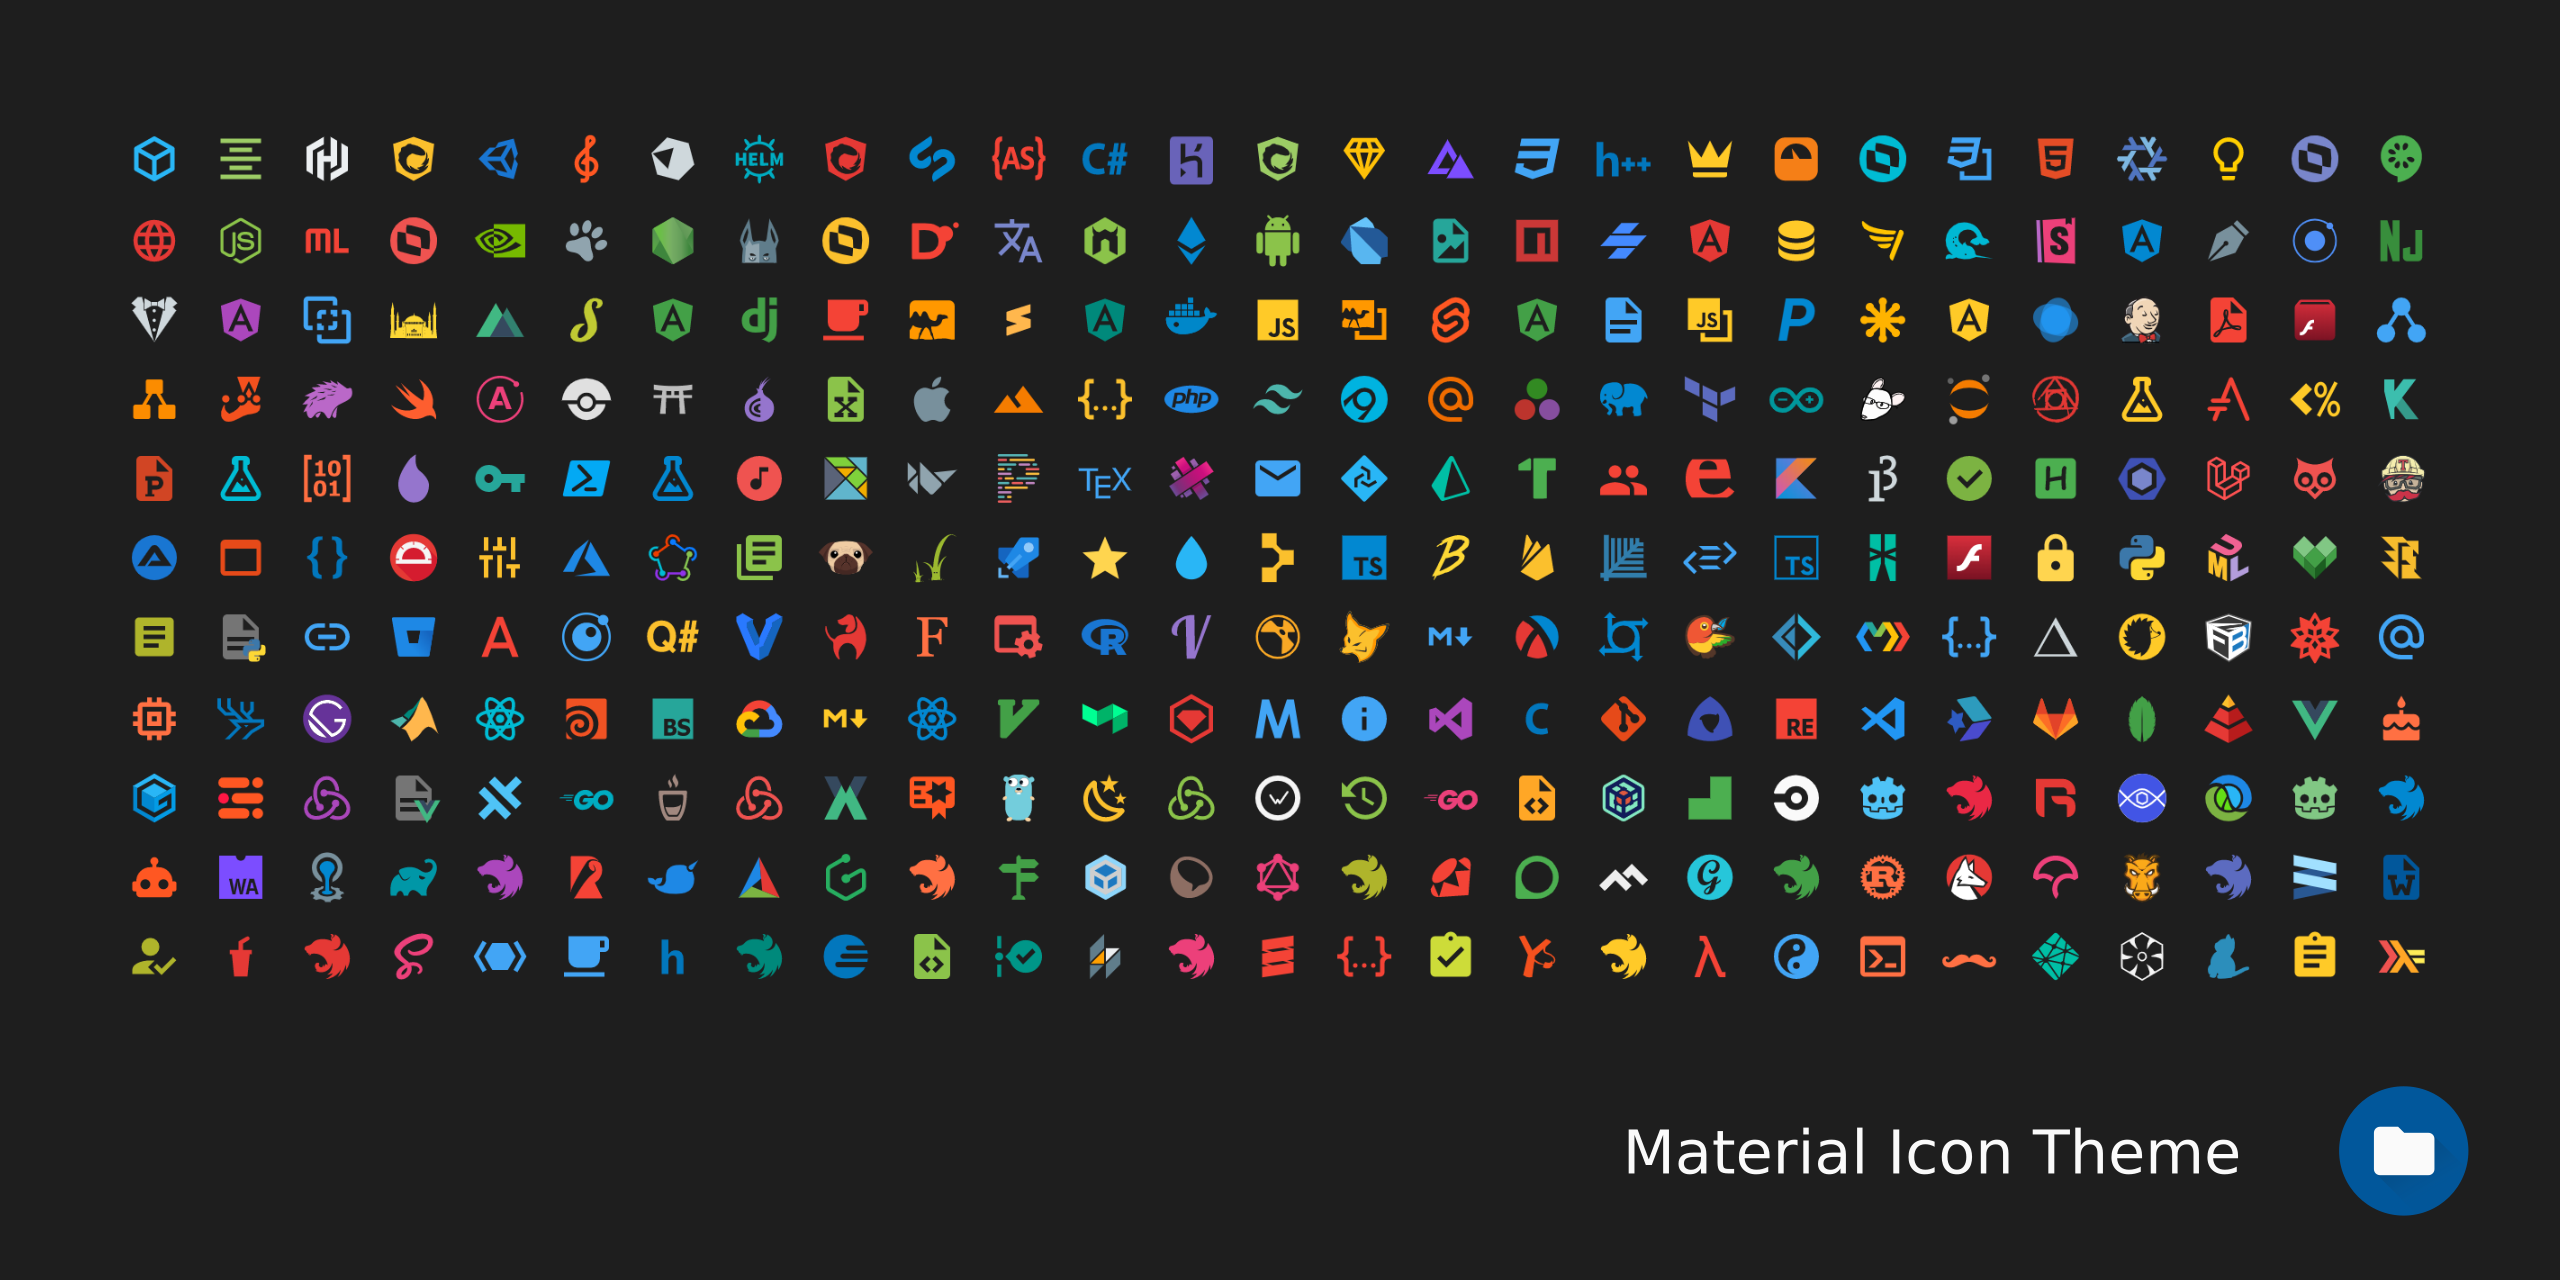
\includegraphics[width=13cm]{images/MaterialIcon.png}
  \caption{Material Icon Theme}
\end{center}
\end{figure}
\item
\textbf{Package Json Upgrade:} Mostra gli aggiornamenti disponibili in package.json. Offre azioni rapide per guidare nell'aggiornamento.
\end{itemize}

\pagebreak
\section{HeidiSQL}
\begin{figure}[ht!]
\begin{center}
  
\includegraphics[width=3cm]{images/HeidiSQL.png}
  \caption{Logo HeidiSQL}
\end{center}
\end{figure}
HeidiSQL è un software gratuito e ha l'obiettivo di essere di facile comprensione, consente di visualizzare e modificare dati e strutture da computer che eseguono uno dei sistemi di database MariaDB, MySQL, Microsoft SQL, PostgreSQL e SQLite. Appartiene agli strumenti più popolari per MariaDB e MySQL in tutto il mondo \cite{HeidiSQL}. Tale strumento è stato utilizzato per la comunicazione con il server, al fine di manipolare le informazioni nei database che il server gestisce.

\section{Microsoft SQL Server Management Studio}
\begin{figure}[ht!]
\begin{center}
  \includegraphics[width=5cm]{images/mssql.png}
  \caption{Logo Microsoft SQL Server Management Studio}
\end{center}
\end{figure}
SQL Server Management Studio (SSMS) è un ambiente gratuito e integrato per la gestione di qualsiasi infrastruttura SQL, da SQL Server al database SQL di Azure. SSMS offre gli strumenti per configurare, monitorare e amministrare le istanze di SQL Server e i database. SSMS viene impiegato per distribuire, monitorare e aggiornare i componenti del livello dati usati dalle applicazioni, nonché per creare query e script.
È possibile usare SSMS per eseguire query, progettare e gestire database e data warehouse in qualsiasi posizione, nel computer locale o nel cloud \cite{MSSQL}.

\pagebreak
\section{Postman}
\begin{figure}[ht!]
\begin{center}
  
\includegraphics[width=4cm]{images/postman_logo.png}
  \caption{Logo Postman}
\end{center}
\end{figure}
Postman è uno strumento di sviluppo di API (application programming interface) che aiuta a costruire, testare e modificare API. Permette di fare vari tipi di richieste HTTP (GET, POST, PUT, PATCH), salvare gli ambienti per usi futuri e convertire le API in codice per vari linguaggi (come JavaScript, Python) \cite{POSTMAN}.
Nel corso dello sviluppo Postman è stato uno strumento essenziale per testare in modo veloce e immediato le richieste HTTP al backend.
\begin{figure}[ht!]
\begin{center}
  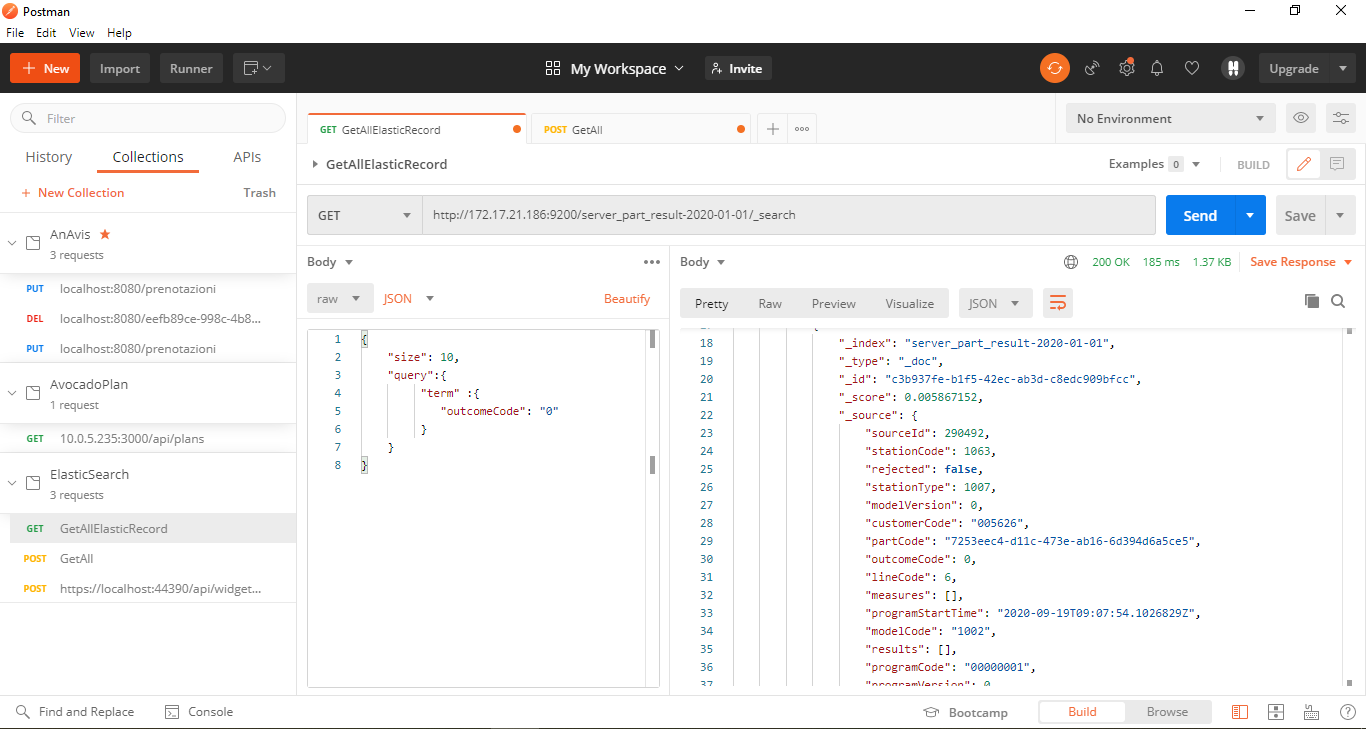
\includegraphics[width=15cm]{images/Postman.png}
  \caption{Schermata di Postman}
\end{center}
\end{figure}

\pagebreak
\section{JMeter}
\begin{figure}[ht!]
\begin{center}
  
\includegraphics[width=6cm]{images/jmeter_logo.png}
  \caption{Logo JMeter}
\end{center}
\end{figure}
\FloatBarrier
Apache JMeter™ è un software open source sviluppato interamente in Java e progettato per fare test di carico e misurare le prestazioni. Originariamente era stato pensato solamente per testare le applicazioni Web, ma nel tempo sono state aggiunte altre funzionalità di testing. 
Può essere utilizzato per testare la resistenza di un server, una rete o un oggetto simulando diversi tipi di carichi pesanti per analizzarne le prestazioni complessive.

Le principali tipologie di applicazioni/server/protocolli che possono essere testate sono:
\begin{itemize}
    \item web - HTTP, HTTPS (Java, NodeJS, PHP, ASP.NET, …)
    \item SOAP / REST Webservices
    \item FTP
    \item database via JDBC
    \item LDAP
    \item message-oriented middleware (MOM) via JMS
    \item mail - SMTP(S), POP3(S) and IMAP(S)
    \item native commands or shell scripts
    \item TCP
    \item Java Objects
\end{itemize}
\cite{JMETER} 
Apache JMeter è stato utilizzato per testare l'applicativo backend del progetto.